\documentclass[12pt]{beamer}
\usepackage{multicol}
\usepackage{amsmath}
\usepackage{mathpazo}
\mode<presentation> 
{
% The Beamer class comes with a number of default slide themes
% which change the colors and layouts of slides. Below this is a list
% of all the themes, uncomment each in turn to see what they look like.

%\usetheme{default}
%\usetheme{AnnArbor}
%\usetheme{Antibes}
%\usetheme{Bergen}
%\usetheme{Berkeley}
%\usetheme{Berlin}
%\usetheme{Boadilla}
%\usetheme{CambridgeUS}
%\usetheme{Copenhagen}
%\usetheme{Darmstadt}
%\usetheme{Dresden}
%\usetheme{Frankfurt}
%\usetheme{Goettingen}
%\usetheme{Hannover}
%\usetheme{Ilmenau}
%\usetheme{JuanLesPins}
%\usetheme{Luebeck}
\usetheme{Madrid}
%\usetheme{Malmoe}
%\usetheme{Marburg}
%\usetheme{Montpellier}
%\usetheme{PaloAlto}
%\usetheme{Pittsburgh}
%\usetheme{Rochester}
%\usetheme{Singapore}
%\usetheme{Szeged}
%\usetheme{Warsaw}

% As well as themes, the Beamer class has a number of color themes
% for any slide theme. Uncomment each of these in turn to see how it
% changes the colors of your current slide theme.

%\usecolortheme{albatross}
\usecolortheme{beaver}
%\usecolortheme{beetle}
%\usecolortheme{crane}
%\usecolortheme{dolphin}
%\usecolortheme{dove}
%\usecolortheme{fly}
%\usecolortheme{lily}
%\usecolortheme{orchid}
% \usecolortheme{rose}
%\usecolortheme{seagull}
%\usecolortheme{seahorse}
%\usecolortheme{whale}
%\usecolortheme{wolverine}

%\setbeamertemplate{footline} % To remove the footer line in all slides uncomment this line
%\setbeamertemplate{footline}[page number] % To replace the footer line in all slides with a simple slide count uncomment this line

%\setbeamertemplate{navigation symbols}{} % To remove the navigation symbols from the bottom of all slides uncomment this line
}

\usepackage{graphicx}
\usepackage{textpos}
\usepackage{tabularx}

\begin{document}

\title[SALSA20]{\vspace{0.15cm} \Large{\textsc{SALSA20}} : Implementation}
\institute[Bibek Ghosh]{

\includegraphics[scale=0.15]{ISI_logo.PNG}

\footnotesize{Indian Statistical Institute, Kolkata}}
\date{April $19^{th}$, 2024}
% \scriptsize{\date{March $19^{th}$, 2024}} 
% Date, can be changed to a custom date


\begin{frame}
\titlepage
\end{frame}

%	TITLE PAGE

\begin{frame}
\frametitle{Contents} 
\begin{multicols}{2}
\tableofcontents
\end{multicols}
\end{frame}

\section{Rise of Salsa20}
\subsection{Background}
\begin{frame}
\frametitle{Background}

\begin{block}{Background}
    \begin{itemize}
    \item Use of network based applications are growing at a rapid speed.
    \item \textit{Pseudo-random} numbers are at the core of any network security application.
    \item \textit{Osvik}, \textit{Shamir} and \textit{Tromer} used cache-timing attacks to steal $AES$ keys from a Linux disk-encryption device.
    \item Serious key collision \& leakage in the hardware implementation of AES ciphers was found.
    \item $A.Shamir$, $I.Mantin$ and $S.fluhrer$ revealed weaknesses in key scheduling algorithm of $RC4$.
    \item Cipher should be \textbf{"GENERIC"} compatible on both Hardware and Software platforms.
\end{itemize}    
\end{block}

This way $Salsa20$ came to the picture
\end{frame}
\subsection{History}

\begin{frame}
\frametitle{Rise of Salsa20}

\begin{block}{History}
\begin{itemize}
    \item $\mathbf{eStream}$ : The $Ecrypt$ Stream Cipher Project, called for submissions of stream ciphers in \textit{November 2004}. 
    \item $\mathbf{Salsa20}$ : Family of $256-bit$ stream ciphers designed in 2005 and submitted to $eStream$ by \textit{Daniel J. Bernstein}.
    \item Salsa20 progressed to the \textit{third round} of $eSTREAM$ without any further changes.
    \item The final $eStream$ portfolio, containing four software stream ciphers and four hardware stream ciphers, were announced in April  \textit{2008}.
    \item It is not \textbf{patented}, and Bernstein has written several public domain implementations optimized for common architectures.
\end{itemize}

\end{block}
\end{frame}


\section{Overview}
\begin{frame}
	
\frametitle{Overview}
\begin{itemize}
    \item Long chain of simple operations, rather than a shorter chain of complicated operations.
    \item This software-oriented stream cipher is built on a $Pseudorandom$ function based on $ADD–ROTATE–XOR$ (ARX) operations.
    \item It undergoes the following set of operations :
    \begin{itemize} 
        \item $\mathbf{32-bit}$ Addition producing the sum $a \ + \ b \ mod 2^{32}$ of two $32-bit$ words $a, \ b$.
        \item $\mathbf{32-bit}$ Exclusive-Or, producing the $a \ \oplus \ b$ of two $32-bit$ words $a, \ b$.
        \item Constant-distance $\mathbf{32}$-bit rotation, producing the rotation $a \ \lll \ b$ of a $32-bit$ word $a$ by $b$ bits to the \textbf{left} (where $b$ is constant).
    \end{itemize}
\end{itemize}
\end{frame}
\subsection{Agility of Salsa20}

\begin{frame}
\frametitle{Agility of Salsa20}
\begin{columns}[c]

\column{.65\textwidth} 
\begin{figure}
    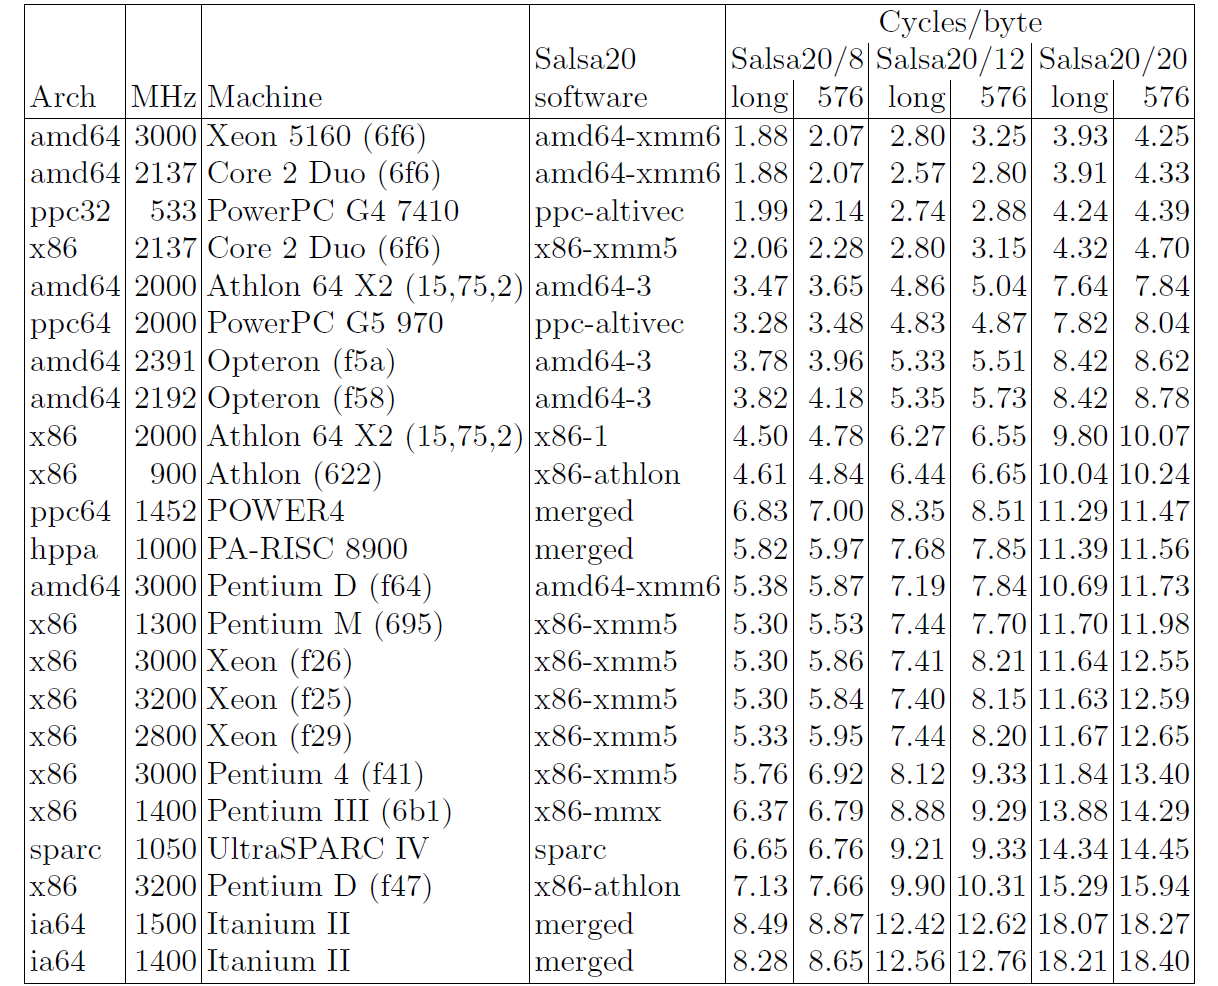
\includegraphics[scale=0.24]{speed.png}
    \tiny{\caption{Speed on different platforms}}
\end{figure}

\column{.55\textwidth}
Where we have : 
\begin{itemize}
    \item \small{${Cycles/byte} \ = $}
    \item[] $\dfrac{cycles \ per \ Sec}{speed}$
    \item \small{${speed = \dfrac{data \ size}{time}}$}
\end{itemize}

\end{columns}

\end{frame}
\subsection{Speed}
\begin{frame}
\frametitle{Speed}

\begin{block}{}
\begin{itemize}
    \item $Salsa20/20$ runs at $3.93$ cycles/byte for long streams. Whereas the fastest $AES$ takes $9.2$ cycles/byte for just $10$ rounds of long stream. 
    \item  $Salsa20$ runs at only $5.14$ cycles/byte on a \textit{Qualcomm Snapdragon S4 processor}, compared to $18.62$ cycles/byte for $AES-128$ in counter mode.
    \item $3$ cycles/byte for \textit{Cryptography} on \textit{Core 2} $Salsa20/12$ rounds takes $2.8$ cycles/byte, one can afford at most $3$ rounds of $AES$ for any security at all.
\end{itemize}    
\end{block}

\end{frame}
\section{Salsa20 Specification}
\subsection{Initial State of $Salsa20$}

\begin{frame}
\frametitle{Initial State of Salsa20}
A \textbf{word} is an element of $\{0,1,\ldots,2^{32} - 1\}$ \\
 The internal state is made of \textbf{sixteen} $32$-bit words arranged in a $4 \times 4$ matrix. The initial state contains \textbf{eight} words of \textit{key} , \textbf{two} words of \textit{stream position} , \textbf{two} words of \textit{nonce} (essentially additional stream position bits), and \textbf{four} \textit{fixed words}:\\
\begin{table}[h!]
\begin{center}
\begin{tabular}{ ||c||c||c||c|| } 
\hline
\hline
"expa" & key & key & key\\
\hline
\hline
key & "nd 3"  & nonce & nonce\\
\hline
\hline
block & block & "2-by" & key\\
\hline
\hline
key & key & key & "te k"\\
\hline
\hline
\end{tabular}

% COLOR EACH CELLS 
\end{center}
\caption{$Salsa20$'s initial state (\textbf{IS}) for $32$ byte keys.}
\end{table}
\end{frame}

\subsection{The Quarterround function}

\begin{frame}
\frametitle{The Quarterround function}

If $x$ is a $4$-word sequence then $quarterround(x)$ is also a $4$-word sequence. 
\begin{block}{Definition}
If $x \ = \ (x_0, \ x_1, \ x_2, \ x_3)$ then ${quarterround(x)} \ = \ (y_0, \ y_1, \ y_2, \ y_3)$ where :
$$y_1 \ = \ x_1 \ \oplus \ ((x_0 \ + \ x_3) \ \lll \ 7)$$
$$y_2 \ = \ x_2 \ \oplus \ ((x_1 \ + \ x_0) \ \lll \ 9)$$ 
$$y_3 \ = \ x_3 \ \oplus \ ((x_2 \ + \ x_1) \ \lll \ 13)$$
$$y_0 \ = \ x_0 \ \oplus \ ((x_3 \ + \ x_2) \ \lll \ 18)$$ 
\end{block}
\textbf{N.B. :} Each modification is \textbf{invertible}, so the entire function is \textbf{invertible}.
\end{frame}
\subsubsection{Diagram}
\begin{frame}
\frametitle{Diagram}

\begin{figure}
    \centering
    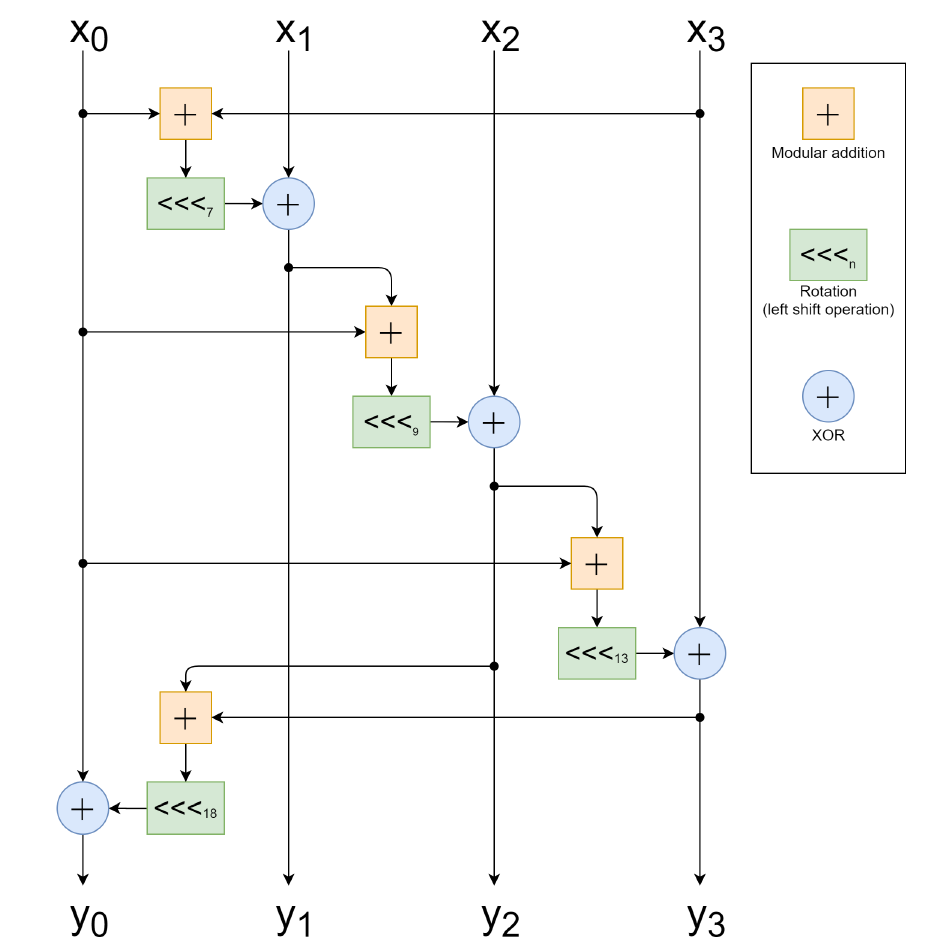
\includegraphics[scale=0.28]{qr.png}
\end{figure}
{\tiny
$\text{quarterround}(0x00000001, \ 0x00000000, \ 0x00000000, \ 0x00000000) = (0x08008145, \ 0x00000080, \ 0x00010200, \ 0x20500000)$
}
\end{frame}
\subsection{The Rowround function}

\begin{frame}
\frametitle{The Rowround function}

If $y$ is a $16$-word sequence then $rowround(y)$ is a $16$-word sequence.

\begin{block}{Definition}
If $y \ = \ (y_0, \ y_1, \ y_2, \ y_3, \ \ldots, \ y_{15})$ then ${rowround(y)} \ = \ (z_0, \ z_1, \ z_2, \ z_3, \ \ldots, \ z_{15})$, where 
$$(z_0, \ z_1, \ z_2, \ z_3) \ = \ quarterround (y_0, \ y_1, \ y_2, \ y_3)$$
$$(z_5, \ z_6, \ z_7, \ z_4) \ = \ quarterround (y_5, \ y_6, \ y_7, \ y_4)$$
$$(z_{10}, \ z_{11}, \ z_8, \ z_9) \ = \ quarterround (y_{10}, \ y_{11}, \ y_{8}, \ y_9)$$
$$(z_{15}, \ z_{12}, \ z_{13}, \ z_{14}) \ = \ quarterround (y_{15}, \ y_{12}, \ y_{13}, \ y_{14})$$
\end{block}
\end{frame}

\subsection{The Columnround function}

\begin{frame}
\frametitle{The Columnround function}

If $x$ is a $16$-word sequence then $columnround(x)$ is a $16$-word sequence. 
\begin{block}{Definition}
If $x \ = \ (x_0, \ x_1, \ x_2, \ x_3, \ \ldots, \ x_{15})$ then ${columnround(x)} = (y_0, \ y_1, \ y_2, \ y_3, \ \ldots, \ y_{15})$ where, 
$$(y_0, \ y_4, \ y_8, \ y_{12}) = quarterround (x_0, \ x_4, \ x_8, \ x_{12})$$
$$(y_5, \ y_9, \ y_13, \ y_1) = quarterround (x_5, \ x_9, \ x_{13}, \ x_1)$$
$$(y_{10}, \ y_{14}, \ y_2, \ y_6) = quarterround (x_{10}, \ x_{14}, \ x_2, \ x_6)$$
$$(y_{10}, \ y_{14}, \ y_{2}, \ y_6) = quarterround (x_{10}, \ x_{14}, \ x_2, \ x_6)$$
\end{block}
\end{frame}
\subsection{The Doubleround function}

\begin{frame}
\frametitle{The Doubleround function}

If $x$ is a $16$-word sequence then $doubleround(x)$ is a $16$-word sequence.
\begin{block}{Definition}
A ${doubleround}$ function is the composition of $columnround$ followed by the $rowround$ function, So we have 
$$doubleround(x)  \ = \ 
rowround(columnround(x))$$
\end{block}
\end{frame}
\subsection{The Littleendian function}

\begin{frame}
\frametitle{The Littleendian function}

If $b$ is a $4$-byte sequence then $littleendian(x)$ is a word.
\begin{block}{Definition}
If b = $(b_0,b_1,b_2,b_3)$ then we have, $${littleendian(b)} \ = \ b_0 \ + \ 2^8 \cdot b_1 \ + \ 2^{16} \cdot b_2 \ + \ 2^{24} \cdot b_3$$
\end{block}
\begin{example}
$$littleendian(255, \ 250, \ 126, \ 96) \ = \ 0x \ \underline{60} \ \underline{7e} \ \underline{fa} \ \underline{ff}$$
$$(255)_{2^{8}} \ = \ (\underline{1111} \ \underline{1111})_2 \ = \ (ff)_{16}$$
$$(250)_{2^{8}} \ = \ (\underline{1111} \ \underline{1100})_2 \ = \ (fa)_{16}$$
$$(126)_{2^{8}} \ = \ (\underline{0111} \ \underline{1110})_2 \ = \ (7e)_{16}$$
$$(96)_{2^{8}} \ = \ (\underline{0110} \ \underline{0000})_2 \ = \ (60)_{16}$$
\end{example}
\end{frame}
\subsection{The Expansion function}
\begin{frame}
\frametitle{The Salsa20 Expansion function}

If $k$ is a $32$-byte and $n$ is a $16$-byte sequence then $Salsa20_k(n)$
is a $64$-byte sequence.
\begin{block}{Definition}
Define $\sigma_0 \ = \ (101, \ 120, \ 112, \ 97)$, $\sigma_1 \ = \ (110, \ 100, \ 32, \ 51)$, $\sigma_2 \ = \ (50, \ 45, \ 98, \ 121)$, and
$\sigma_3 \ = \ (116, \ 101, \ 32, \ 107)$. If $k_0, \ k_1, \ n$ are $16$-byte sequences then we have : $$Salsa20_{k_0,k_1} (n) \ = \ Salsa20(\sigma_0, \ k_0, \ \sigma_1, \ n, \ \sigma_2, \ \ k_1, \ \sigma_3)$$
\end{block}
\begin{exampleblock}{}
\textbf{N.B. :} Expansion refers to the expansion of (k, n) into $Salsa20_k(n)$.
The constants  $\sigma_0$ $\sigma_1$ $\sigma_2$ $\sigma_3$ is "$expand \ 32-byte \ k$" in \textbf{ASCII}.
\end{exampleblock}
\end{frame}
\subsection{The Hash function}
\begin{frame}
\frametitle{The $Salsa20$ Hash function}

If $x$ is a $64$-byte sequence then $Salsa20(x)$ is a $64$-byte sequence. 
\begin{block}{Definition}
$$Salsa20(x) \ = \ x \ + \ doubleround^{10}(x)$$ 
Where each $4$-byte sequence is viewed as a word in $little-endian$ form. 
Starting with $x \ = \ (x[0], \ x[1], \ \ldots, \ x[63])$. Lets, define
\vspace{-8pt}
\[
\begin{gathered}
x_0 \ = \ \text{littleendian}(x[0], \ x[1], \ x[2], \ x[3]) \\
\vdots \\
x_{15} \ = \ \text{littleendian}(x[60], \ x[61], \ x[62], \ x[63])
\end{gathered}
\]
\end{block}
\begin{exampleblock}{}
Define $(z_0, \ z_1, \ \ldots, \ z_{15}) \ = \ doubleround^{10}(x_0, \ x_1, \ \ldots, \ x_{15})$ \\ Then $Salsa20(x)$ is the concatenation of : 
\footnotesize{$$littleendian^{-1}(z_0 + x_0) \ || \ littleendian^{-1}(z_1 + x_1) \ || \ldots || \ littleendian^{-1}(z_{15} + x_{15})$$}
\end{exampleblock}
\end{frame}
\subsection{The Encryption function}
\begin{frame}
\frametitle{The Salsa20 Encryption function}

\begin{exampleblock}{}
\begin{itemize}
    \item Let $k$ be a $32$-byte sequence of key, $v$ be a $8$-byte sequence of nonce and $m$ be an $\textit{l}$-byte sequence of input, (for some $\textit{l} \in \{0,1,\ldots, 2^{70} \}$).
    \item The $Salsa20$ \textit{Encryption/Decryption} of \textit{Input} is denoted by $\mathbf{Salsa20_k(v) \ \oplus \ m}$, is an \textit{l}-byte sequence.
\end{itemize}
\end{exampleblock}
\begin{block}{Definition}
$Salsa20_k(v)$ is a $2^{70}$-byte sequence
\vspace{-5pt}
$$Salsa20_k(v,0) \ || \ Salsa20_k(v,1) \ || \ \ldots \ || \ Salsa20_k(v,2^{64}- 1)$$
$Salsa20_k(v)\oplus m$ implicitly truncates $Salsa20_k(v)$ to the same length as m. In other words : \small{(where $ c[i] = m[i] \oplus Salsa20_k(v, \lfloor\frac{i}{64}\rfloor)[i~ mod 64]$)}
\vspace{-5pt}
  $$Salsa20_k(v) \oplus (m[0],m[1],\ldots,m[l-1]) = (c[0], c[1],\ldots, c[l-1])$$  
\end{block}

\end{frame}
\section{Cryptanalysis on Salsa20}
\subsection{Brute Force Attacks}
\begin{frame}
\frametitle{Brute-force attacks}
The Quarterround ($QR$) function takes a $128$ bit binary number. The total possible combinations of inputs are $2^{128}$.

\begin{alertblock}{}
    A complete search would thus take about: \small{(Assuming we can know the cryptographic nonce used)}
    $$\dfrac{2^{128} QR}{10000 QR/s} \ = \ 3.4 \cdot 10^{34} \ \text{seconds} \ \approx \ 10^{27} \ \text{years}$$
\end{alertblock}

\begin{alertblock}{}
    A complete search of the $256$ bit key space would take:
   $$\dfrac{2^{256} runs}{14 runs/s} \ = \  2.4 \cdot \ 10^{76} \ \text{seconds} \ \approx \ 10^{68} \ \text{years}$$
\end{alertblock}
\end{frame}
\subsection{Hamming distance differential analysis}

\begin{frame}
\frametitle{Hamming distance differential analysis}
For an \textit{Encryption function }$f : f(X) \ \rightarrow \ Y$ \\
If $HD(X, \ X^\prime) \ = \ n$, then $HD(Y, \ Y^\prime) \ \stackrel{?}{=} \ m$
\setlength{\columnsep}{-30pt}
\begin{multicols}{2}
\setlength{\leftmargin}{1pt}
\begin{figure}
    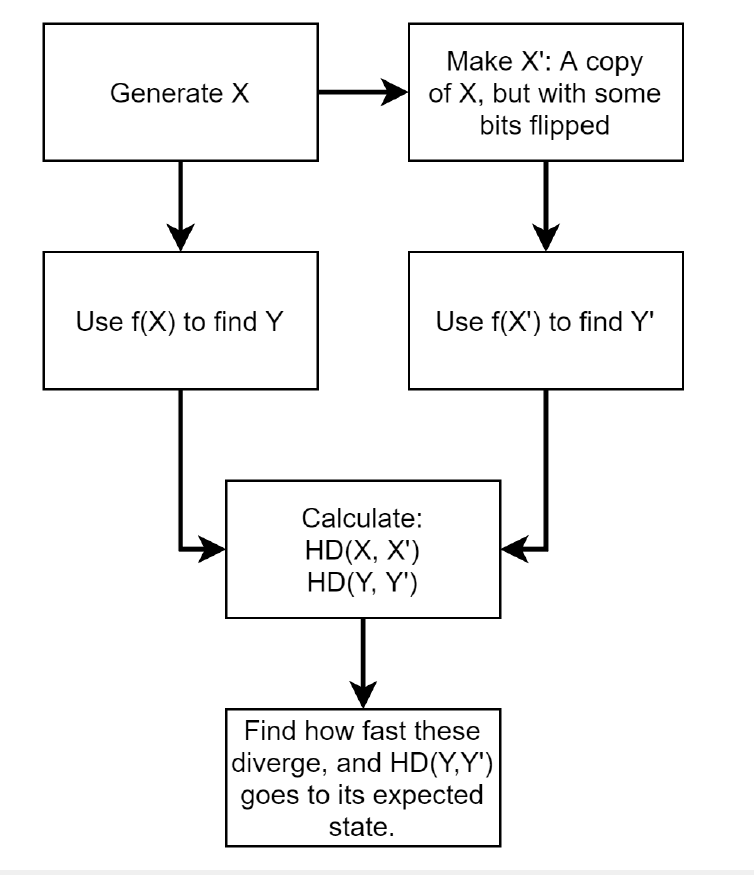
\includegraphics[scale=0.25]{HD.png}
    \tiny{\caption{Hamming Distance}}
\end{figure}
\columnbreak
\begin{itemize}
    \item If the algorithm has a good avalanche effect, we would expect the $HD$ to be about the same as the $HD$ between two random values: About half the bits.
    \item If $P$ and $Q$ are two random binary numbers of length $n$, we would expect: $HD(Q,P) \ \approx \ \dfrac{n}{2}$
\end{itemize}
\end{multicols}
\end{frame}
\subsection{Differential analysis on QR function}
\begin{frame}
\frametitle{Differential analysis on QR function}
As $QR(X)\rightarrow y$ and we get $X^\prime$ by flipping some random bits of $X$. \\
As $n$ increases, $m$ tend towards the expected equilibrium of half the length of $Y$. Analysis based on measuring $HD ( QR (x^\prime), \ y)$ : 


\setlength{\columnsep}{10pt}
\begin{multicols}{2}
\setlength{\leftmargin}{1pt}

{\begin{itemize}
    \item \small{The bit flipping is given by $x$-axis. i.e. $n$ times.}
    \item \small{The $HD$ between $2$ values are given by $y$-axis.}
    \item \small{Legend of the Plot : }
    \begin{enumerate}
    \setcounter{enumi}{-1} % Set the counter to start from 0
        \item  \scriptsize{$HD(X,Y)$}
        \item  \scriptsize{Convergence point of the Hamming distance between two random values}
        \item \scriptsize{$HD(Y,Y^\prime)$}
        \item \scriptsize{$HD(X,X')$}
        \item[] \scriptsize{Assuming $HD(X,X^\prime) < \ \frac{key \ size}{8}$, $HD(X,\ X^\prime)$ should be easily distinguishable.}
    \end{enumerate}
\end{itemize}}

\columnbreak
\setlength{\rightmargin}{0pt}
\begin{figure}
    \centering
    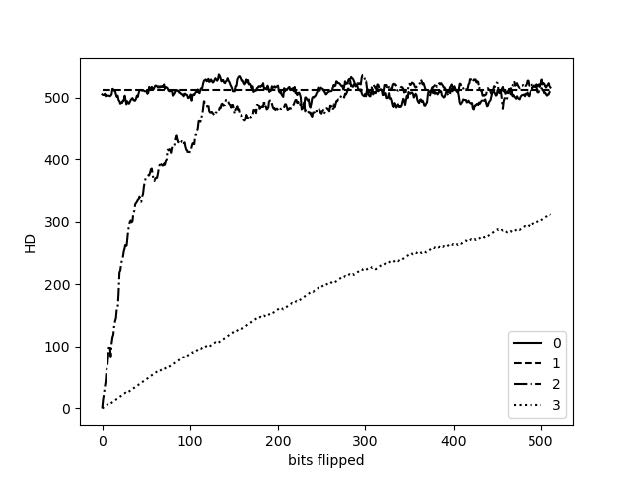
\includegraphics[scale=0.52]{fig1.jpg}
    \caption{Flipping of random bits in $X$}
\end{figure}

\end{multicols}

\end{frame}
\begin{frame}
\frametitle{Contd.}

\setlength{\columnsep}{10pt}
\begin{multicols}{2}
\setlength{\leftmargin}{1pt}
\setlength{\rightmargin}{0pt}
\begin{figure}
    \centering
    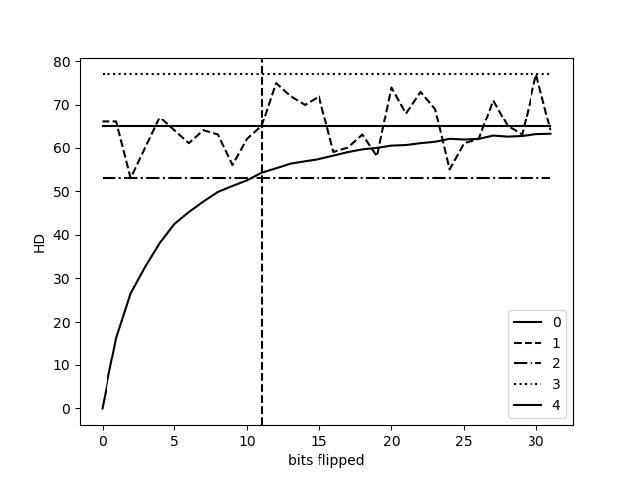
\includegraphics[scale=0.55]{fig2.jpg}
    \caption{Averaging of effects on $Y$ when bits are 
flipped in $X$.}
\end{figure}

\columnbreak
Legend of the Plot : 
\begin{enumerate}
    \setcounter{enumi}{-1} % Set the counter to start from 0
    \item \footnotesize{$HD(X^\prime, Y^\prime)$ as $n$ bits in $X^\prime$ are flipped.}
    \item \footnotesize{$HD(X,Y)$ of random $X$s}
    \item \footnotesize{\textit{Minimum expected difference} between two random $X$s}
    \item \footnotesize{\textit{Maximum expected difference} between two random $X$s}
    \item \footnotesize{\textit{Expected average difference} between two random $X$s}
    \item[] \footnotesize{The vertical line is where the bits flipped needed for the Hamming distance to be within the range of expected random distances}
\end{enumerate}
\end{multicols}
\end{frame}
\subsection{Analysis on Salsa20’s PRG}
\begin{frame}
\frametitle{Analysis on Salsa20's PRG}

\setlength{\columnsep}{10pt}
\begin{multicols}{2}
\setlength{\leftmargin}{1pt}

{\begin{itemize}
    \item \small{Line $1$, shows how, $HD(input_{original}, \ input_{next})$ is roughly equal to $1$ per flipped bits.}
    \item \small{Line $2$, is the expected value for random inputs and outputs.}
    \item \small{Line $0$, seems to be no correlation or pattern between the amounts of bits flipped in the $input(n)$ and the $HD$ between the two values.}
\end{itemize}}

\columnbreak
\setlength{\rightmargin}{0pt}
\begin{figure}
    \centering
    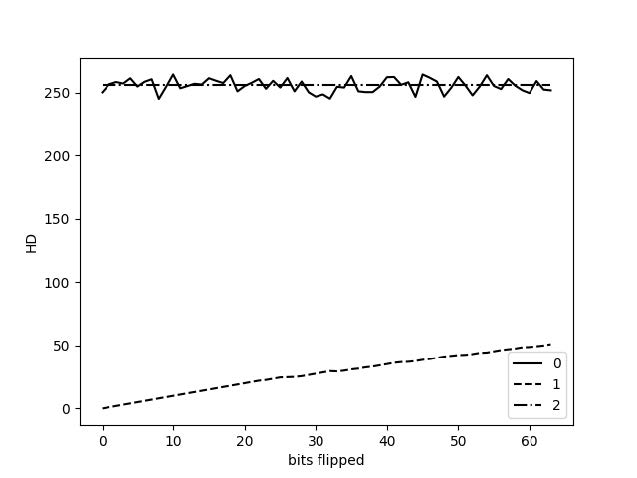
\includegraphics[scale=0.55]{fig3.jpg}
    \caption{Averaging of effects on the $PRG$ output when bits are 
flipped in key}
\end{figure}

\end{multicols}

\end{frame}
\section{The Invincible Salsa20}

\begin{frame}
\frametitle{The Invincible Salsa20}
\begin{alertblock}{}
    $Salsa20$ is highly resistant and secure against all the well known attacks : 
    \begin{itemize}
        \item $Algebraic$ attack
        \item $Weak-Key$ attack
        \item $Equivalent-Key$ attack
        \item $Related-Key$ attack
        \item $Correlation \ power \ analysis$
        \item $Context \ aggregation$ network analysis
    \end{itemize}
\end{alertblock}

\end{frame}
\section{Conclusion}

\begin{frame}
\frametitle{Conclusion}
\begin{alertblock}{}
    After going through all this discussions, we conclude with the following points : 
    \begin{itemize}
        \item $SALSA20$ is faster and efficient as compared to $AES$.
        \item Been secure to both $KPA$ and $CPA$.
        \item Efficient in both \textit{software} and \textit{hardware}.
        \item \textit{Brute force} attack are not easily implementable.
    \end{itemize}
\end{alertblock}

\end{frame}
\section{References}

\begin{frame}
\frametitle{References}

\begin{thebibliography}{100}
\bibitem{Bernstein2008} D. J. Bernstein, \emph{“The Salsa20 Family of Stream Ciphers”}, New Stream Cipher Des., pp. 84–97, 2008.
\bibitem{Bernstein2005} D. J. Bernstein, \emph{“Salsa20 specification”}, eSTREAM Proj. algorithm Descr., pp. 2–10, 2005.
\bibitem{StackExchange2012} "Calculating cycles per byte." Stream cipher - Calculating cycles per byte - Cryptography Stack Exchange. N.p., 2 Oct. 2012. Web. 3 Mar. 2017. \newline \url{http://crypto.stackexchange.com/questions/3943/calculating-cycles-per-byte} 
\bibitem{StackExchange2016} "How secure is Salsa20?" Algorithm design - How secure is Salsa20? - Cryptography Stack Exchange. N.p., 8 Oct. 2016. Web. 10 Mar. 2017. \newline \url{http://crypto.stackexchange.com/questions/40542/how-secure-is-salsa20/40543} 

\end{thebibliography}
\end{frame}



\end{document} 